\chapter{関連研究}

\section{Neural Turing Machine}
NTMの構造を図\ref{fig:ntm}に示す。NTMの構造は3つのコンポーネントに分けられる。
\\1.情報を保存するメモリ$M_t$は$N×W$次元の行列からなり、これは$W$次元の項目を$N$スロット分保存できる。
\\2.コントローラは毎時間ステップで入力$x_t$を受け取り、隠れ状態$h_t$を計算する。
任意のRNNがコントローラとして採用可能であるが、大抵LSTMが用いられる。
\\3.読み出し/書き込みヘッドはコントローラ出力$h_t$とメモリ$M_t$の内容から読み出し/書き込み重みを計算し、メモリへの読み書きを行う。
読み出し/書き込み重みはそれぞれ各スロットへの書き込み/読み出しの強度を表す$N$次元のアテンション係数である。
この重みを計算する操作を”アドレス指定”操作と呼ぶ。

2.1.1節ではヘッドにおける読み書きを説明する。2.1.2節ではアドレス指定を説明する。

\begin{figure}[t]
	\centering
	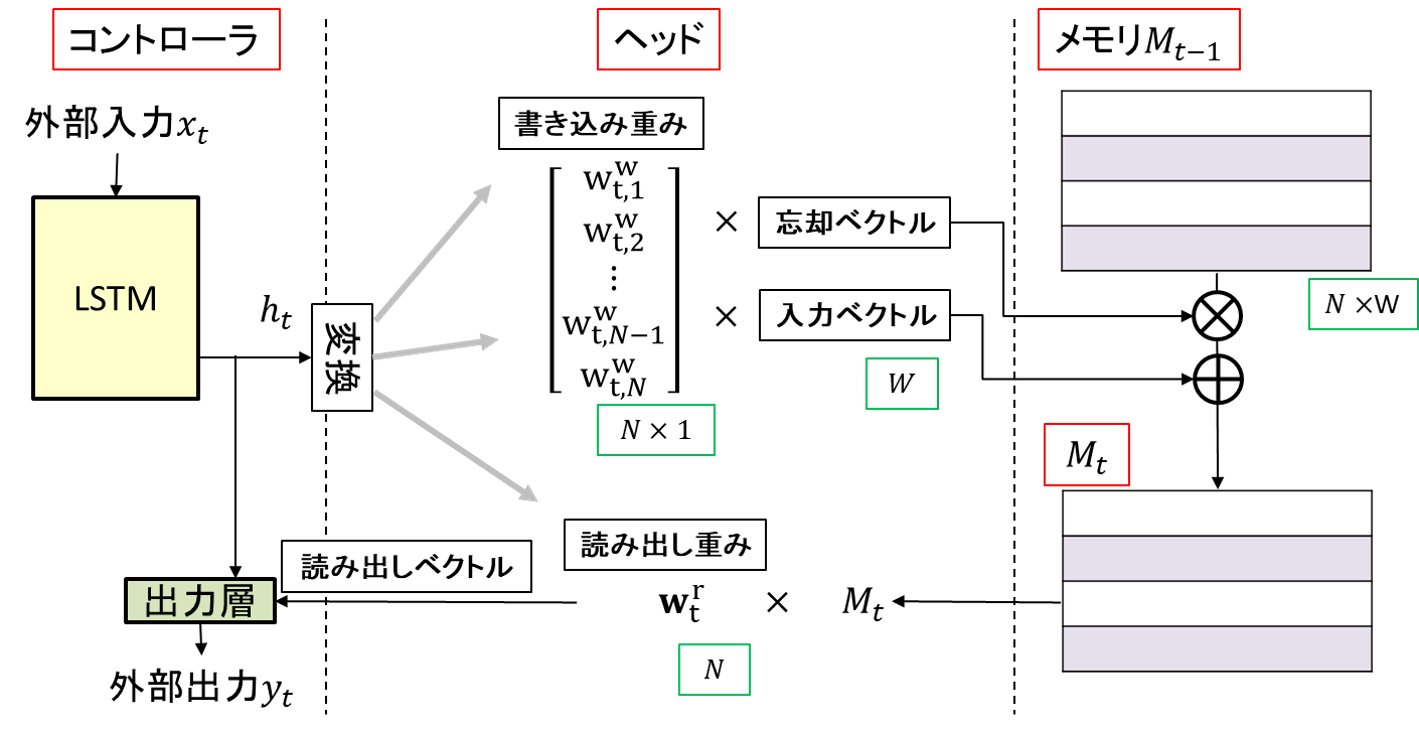
\includegraphics[width=\linewidth]{./figure/img_slide/ntm.png}
	\caption{NTMの構造}
	\label{fig:ntm}
\end{figure}

\subsection{読み出し/書き込みヘッド}
NTMは読み出し用のヘッドと書き込み用のヘッドそれぞれを1つ以上持ち、ヘッドごとにアドレス指定及び読み書きが行われる。
読み/書き重みをそれぞれ$w^r_t$,$w^w_t$と表し、これらは2.1.2節で説明するアドレス指定操作を用いて計算される。
$w^r_t$,$w^w_t$は式\ref{eq:att1},\ref{eq:att2}を満たすアテンション係数である。
\begin{equation} \label{eq:att1}
	\sum_{i}w_t(i) = 1
\end{equation}
\begin{equation} \label{eq:att2}
	0\leq w_t(i)\leq 1 , \forall i
\end{equation}
ここで$w_t(i)$は$w_t$のi番目の要素である。
メモリからの読み出しは式\ref{eq:readv}のように計算され、読み出しベクトル$r_t$を得る。
\begin{equation}\label{eq:readv}
	r_t = \sum_{i}w^r_t(i)M_t(i)
\end{equation}
$M_t(i)$は$M_t$のi行目を表す。書き込みは式\ref{eq:ntm_forg}による忘却、式\ref{eq:ntm_add}による加算の順で計算され、$M_{t-1}$を$M_t$に更新する。
忘却ベクトル$e_t$、書き込みベクトル$a_t$はコントローラ出力からの変換で得られる。ただし忘却ベクトルの各要素は(0,1)の範囲にある。
\begin{equation} \label{eq:ntm_forg}
	M_t'(i) = M_{t-1}(i)[1-w^w_t(i)e_t]
\end{equation}
\begin{equation} \label{eq:ntm_add}
	M_t(i) = M_t'(i) + w^w_t(i)a_t
\end{equation}

\subsection{アドレス指定操作}
読み書きの重み$w_t$は2つの異なるコンセプトに基づいて算出された重みから計算される。
類似するメモリ内容を参照するコンテンツベースの重み$w^c_t$と,メモリの各行を位置によって役割を分ける位置ベースの重み$s_t$である。
アドレス指定操作の中で用いられる$k_t$,$\beta_t$,$s_t$,$g_t$,$\gamma_t$はコントローラ出力$h_t$からの変換で計算される。

はじめにコンテンツベースの重み$w^c_t$は式\ref{eq:w_content}に示すように,キーベクトル$k_t$とメモリ各行の類似度に基づいて計算される。
\begin{equation} \label{eq:w_content}
	w^c_t(i) =\frac{\exp(\beta_tK\left[k_t,M_t(i)\right] ) }{\sum_j\exp(\beta_tK\left[k_t,M_t(j)\right] )}  
\end{equation}
キー強度$\beta_t$は正の値を取り,$K[.,.]$はコサイン類似度の計算を表す。
$w^c_t$と前の時間ステップでの重み$w_{t-1}$を式\ref{eq:w_interp}によって補間し、$w^g_t$を得る。
\begin{equation} \label{eq:w_interp}
	w^g_t(i) = g_t w^c_t+(1-g_t)w^w_{t-1}
\end{equation}
$g_t$は(0,1)の範囲にあるスカラー値である。

次にこの重みと位置ベースの重み$s_t$の畳み込み計算を式\ref{eq:w_shift}行う。
この畳み込みは式\ref{eq:w_interp}で注目した場所からの位置のシフトを表現している。
例えば前の時間ステップで書き込んだ位置の下に書き込み位置をずらしたり、類似した項目の隣の情報を読み出す機能を実現する。
\begin{equation} \label{eq:w_shift}
	\tilde{w_t}(i) = \sum_{j=0}^{N-1}w^g_t(j)s_t(i-j)
\end{equation}

ここまでの操作で計算されたアテンション係数では重みが複数の位置に分散し,内容が拡散してしまう可能性がある。最後に式\ref{eq:w_sharp}を適用して重みをシャープにし,ヘッドが作用するメモリ行を限定する。
\begin{equation} \label{eq:w_sharp}
	w_t(i) = \frac{\tilde{w_t}(i)^{\gamma_t}}{\sum_j\tilde{w_t}(j)^{\gamma_t}}
\end{equation}

\section{Relational Memory Core}
関係メモリのベースとして使用した、\cite{rrnn}で提案されたRMCを説明する。RMCの構造を図\ref{fig:rmc}に示す。

\begin{figure}[t]
	\centering
	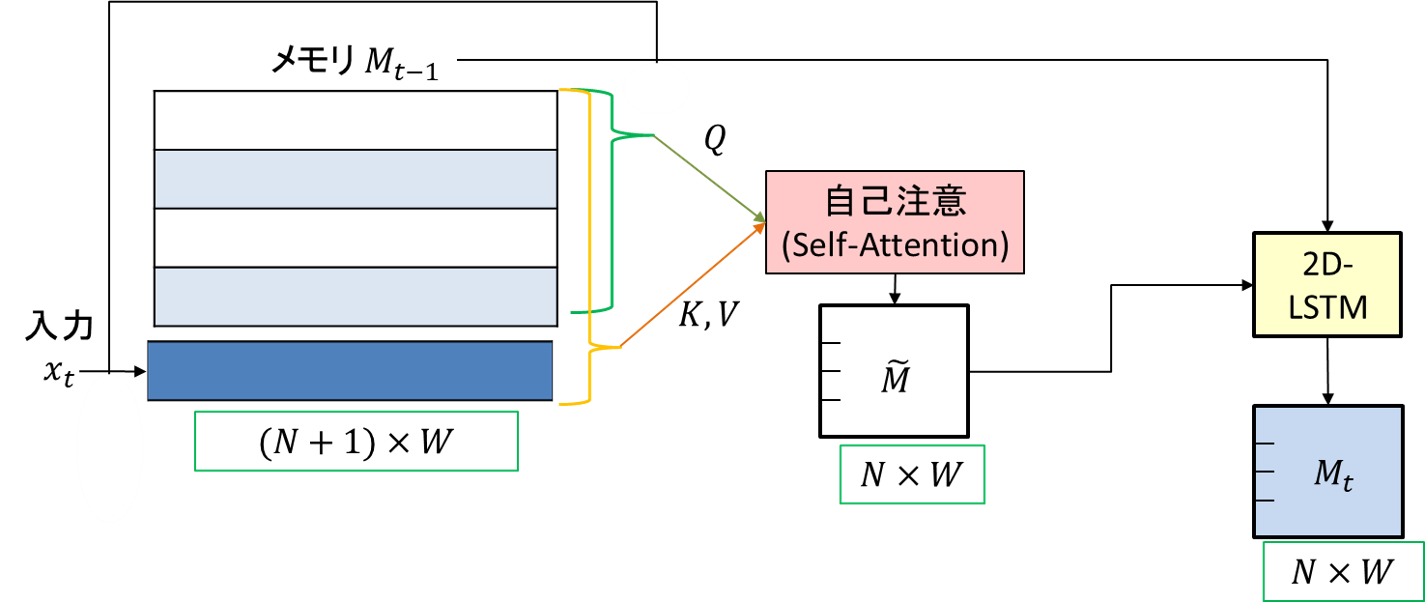
\includegraphics[width=\linewidth]{./figure/img_slide/rmc.png}
	\caption{RMCの構造}
	\label{fig:rmc}
\end{figure}

RMCは毎ステップで入力$x_t$とメモリ$M_{t-1}$の各項目間の関係情報を計算し、そのステップでのメモリ成分$\tilde{M}$を用意する。
LSTMベースのゲーティングを利用して、$\tilde{M}$を$M_{t-1}$に合成し$M_t$を得る。
$\tilde{M}$の計算はマルチヘッドドット積アテンション\cite{transformer}を用いて行われる。
RMCは項目メモリ$M_i$と入力$x_t$からアテンションを計算するために、クエリ・キー・バリューを計算する為の訓練可能な線形層を有する。
それぞれを$W_q$,$W_k$,$W_v$と表現すると、$\tilde{M}$は式\ref{eq:rmc_mtil}のようにして計算される。
\begin{equation} \label{eq:rmc_mtil}
	\tilde{M} =softmax ( \frac{M_{t-1}W_q ([M_{t-1};x_t]W_k)^T}{ \sqrt{d_k}} ) [M_{t-1};x_t]W_v
\end{equation}
ここで$d_k$はキーベクトルの次元 、[M;x]は$M$に$x_t$を新たな行として連結した$(N+1)\times M$次元の行列を表す。クエリ行列の計算では[M:x]ではなく$M$を入力することに注意が必要である。これは$\tilde{M}$の次元を$M_t$と等しくすることを目的としている。

ヘッドが複数存在する時は、ヘッドごとに独立な線形層を用いたアテンション計算結果を結合し最終的な$\tilde{M}$を得る。
各ヘッドの計算結果を$\tilde{M_1},\tilde{M_2}…\tilde{M_h}$と表すとき、それぞれの次元は$N\times (M/h)$であり、$\tilde{M_t}=[\tilde{M_1}: … :\tilde{M_h}]$とすることで$M_t$と同じ次元の$\tilde{M}$を得る。
[:]は行方向の連結を表す。

$\tilde{M}$により$M_t$を更新するためにLSTMを利用する。
$M_t$の各行を2D-LSTMの各メモリセルとして実装することで、式\ref{eq:rmc_l1}-\ref{eq:rmc_l7}によって更新される。
$m_i$,$\tilde{m_i}$はそれぞれ$M_t$,$\tilde{M}$の$i$番目の行を表す。
\begin{equation}\label{eq:rmc_l1}
	s_{i,t}=(h_{i,t-1},m_{i,t-1})
\end{equation}
\begin{equation}\label{eq:rmc_l2}
	f_{i,t}=W^f x_t +U^f h_{i,t-1}+b^f
\end{equation}
\begin{equation}\label{eq:rmc_l3}
	i_{i,t}=W^i x_t +U^i h_{i,t-1}+b^i
\end{equation}
\begin{equation}\label{eq:rmc_l4}
	o_{i,t}=W^o x_t +U^o h_{i,t-1}+b^o 
\end{equation}
\begin{equation}\label{eq:rmc_l5}
	m_{i,t}=\sigma(f_{i,t}+\bar{b}^f)\circ m_{i,t-1}+\sigma(i_{i,t})\circ \underbrace{g_\psi(\tilde{m}_{i,t})}
\end{equation}
\begin{equation}\label{eq:rmc_l6}
	h_{i,t}=\sigma(o_{i,t})\circ \tanh(m_{i,t})
\end{equation}
\begin{equation}\label{eq:rmc_l7}
	s_{i,t+1}=(m_{i,t},h_{i,t})
\end{equation}
式\ref{eq:rmc_l5}において下線部が示す箇所はLSTMからの変更部分である。関数gは既存研究\cite{rrnn}に従い、MLP + layer normalizationとして実装した。パラメータ は各$m_i$について共通する。
